\documentclass[a4paper]{article}
\usepackage{geometry}
\usepackage{multicol}
\usepackage{setspace}
\usepackage{listings}
\usepackage{graphicx}
\usepackage{algorithm}
\usepackage{algorithmic}
\usepackage{amsmath}
\usepackage{multicol}
\usepackage{float}
\DeclareGraphicsExtensions{.eps,.ps,.jpg,.bmp}
\usepackage{xcolor}
%\setlength{\parskip}{0.5\baselineskip}
\geometry{left=3.0cm,right=2.5cm,top=1.0cm,bottom=2.0cm} 
\title{\textbf{Algorithmn HW2}}
\author{5140379032 JIN YI FAN}
\date{}
\begin{document}\large
\maketitle
\begin{spacing}{1.3}
\begin{multicols}{2}
\section*{Problem 1.17}
Construct $f(n)$ and $g(n)$ such that: 
\begin{align}
\frac{\sqrt{2}}{2}(f(n)-x)&=\sin(\frac{\sqrt{2}}{2}(f(n)+x)) \notag \\ 
\frac{\sqrt{2}}{2}(g(n)-x)&=\cos(\frac{\sqrt{2}}{2}(g(n)+x))  \notag
\end{align}
which are shown in axis below, obviously they are neither the other's upper bound.
\begin{figure}[H]
    \centering
    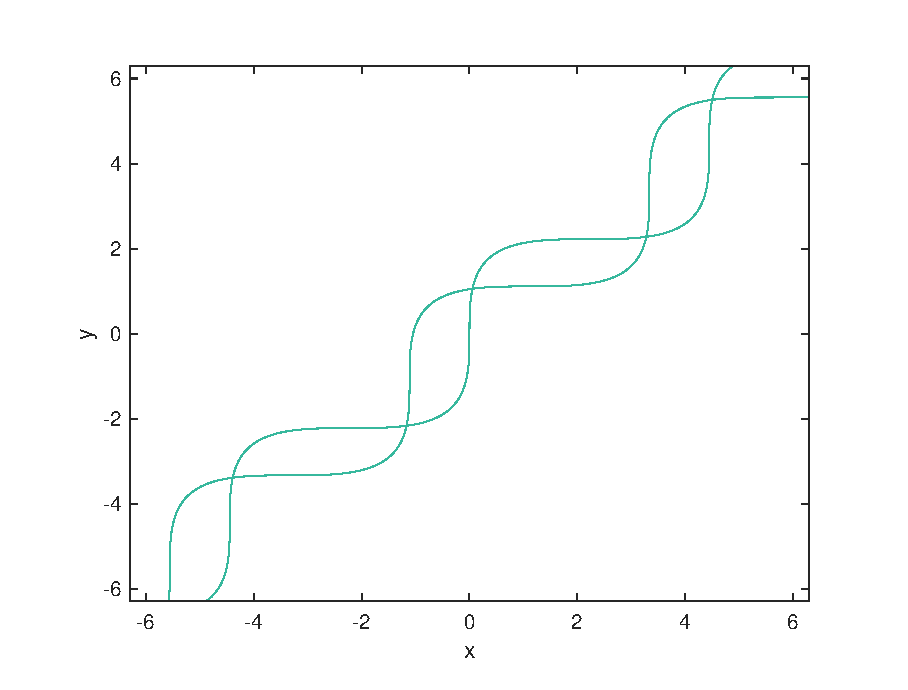
\includegraphics[width=7cm]{graph.eps}
\end{figure}

\section*{Problem 1.34}
\subsection*{(a) $O(n)$}
\begin{algorithmic}[1]
\STATE $MAX \leftarrow A[0]$
\STATE $MIN \leftarrow A[0]$
\FOR{$i = 0$ to $n$}
\STATE $MAX \leftarrow max\{MAX, A[i]\}$
\STATE $MAX \leftarrow min\{MIX, A[i]\}$
\STATE $i \gets i+1$
\ENDFOR
\end{algorithmic}

\subsection*{(b) $\Omega(nlogn)$}
\begin{algorithmic}[1]
\STATE QuickSort($A[]$)
\STATE $MAX \gets A[n]$
\STATE $MIN \gets A[0]$
\end{algorithmic}

\section*{Problem 1.35}
\begin{algorithmic}[1]
\ENSURE no duplicated elements in $A[]$
\STATE $a \leftarrow A[0], b\leftarrow A[1], c\leftarrow A[2]$
\STATE $B[]$=Sort($a,b,c$)
\RETURN $B[1]$
\end{algorithmic}

\section*{Problem 1.37}
Construct an array $P[]$, s.t.$P[i]=a_i$
\subsection*{(a) $\Omega(n^2)$}
\begin{algorithmic}[1]
\STATE $sum \gets P[0]$
\FOR{$i = 1$ to $n$}
\STATE $exp \gets 1$
{\FOR{$j = 1$ to $i$}
\STATE $exp \gets exp*x$
\STATE $j\gets j+1$
\ENDFOR}
\STATE $sum\gets sum+exp*P[i]$
\STATE $i\gets i+1$
\ENDFOR
\RETURN $sum$
\end{algorithmic}

\subsection*{(b) $O(n)$}
\begin{algorithmic}[1]
\STATE $sum \gets P[n]$
\FOR{$i = n-1$ to $0$}
\STATE $sum\gets sum*x+P[i]$
\STATE $i\gets i-1$
\ENDFOR
\RETURN $sum$
\end{algorithmic}

\section*{}
\section*{Problem 2: Egg drop}
\textbf{Version 0:}
\begin{algorithmic}[1]
\REQUIRE 1 egg, $\leq T$ tosses
\STATE{$floor \gets 1$}
\FOR{$floor=1$ to $N$}
\IF{$egg.drop(floor)==break$} \RETURN $floor$ \ENDIF
\STATE $floor \gets floor+1$
\ENDFOR
\RETURN $floor$
\end{algorithmic}

\subsection*{}
\textbf{Version 1:}
\begin{algorithmic}[1]
\REQUIRE $logN$ eggs, $logN$ tosses
	\STATE{$low \gets 1$}
	\STATE{$high \gets N$}
	\STATE{$floor \gets 1$}
\FOR{$i=1$ to $logN$}
	\STATE{$floor \gets low+\frac{high-low}{2}$}
	\IF{$egg.drop(floor)==break$}
	\IF{$high==low$} 
	\RETURN $high$ \ENDIF
	\STATE{$high \gets floor$}
	\ELSE 
	\IF{$high-low\leq 1$} 
	\RETURN $high$ \ENDIF
	\STATE{$low \gets floor$}
	\ENDIF
\ENDFOR
\end{algorithmic}

\subsection*{}
\textbf{Version 2:}
\begin{algorithmic}[1]
\REQUIRE $logT$ eggs, $2logT$ tosses
\STATE{$floor \gets 1$}
\REPEAT
\STATE{$floor \gets (floor*2)$}
\UNTIL{$egg.drop(floor)==break$}
\STATE{$low \gets (floor/2)$}
\STATE{$high \gets floor$}
\STATE{BinaryEggDrop($low$, $high$)}
\COMMENT{The algorithmn starting at Version 1, line $3$}
\end{algorithmic}

\subsection*{}
\textbf{Version 3:}
\begin{algorithmic}[1]
\REQUIRE $2$ eggs, $2\sqrt{T}$ tosses
\STATE{$floor \gets 1$}
\REPEAT
\STATE{$floor \gets (floor+\sqrt{T})$}
\UNTIL{$eggOne.drop(floor)==break$}
\COMMENT{At most $\sqrt{T} tosses$}
\FOR{$i \gets (floor-\sqrt{T})$ to $floor$}
\IF{$eggTwo.drop(i)==break$}
\RETURN $i-1$
\ELSE \STATE{$i\gets i+1$}
\ENDIF
\COMMENT{At most $\sqrt{T}$ tosses}
\ENDFOR
\end{algorithmic}

\subsection*{}
\textbf{Version 4:}
\begin{algorithmic}[1]
\REQUIRE $2$ eggs, $\leq c\sqrt{T}$ tosses
\STATE Don't know how to do it...
\STATE Maybe DP?
\end{algorithmic}
\end{multicols}
\end{spacing}
\end{document}